\chapter{Stitching of Images}

\section{About the Chapter}

The part of image processing in this project is to take the hyperspectral images from the drone and stitch them into a complete image of the farm for further analysis.

We require a well-structured dataset for the proper functioning of this system. The dataset consists of hyperspectral images order to get information about the image on a wider range of spectrum. The dataset should consist of a serial of overlapping images taken of the farm field in all four directions. Overlapping is an essential condition as we require it to increase the accuracy of image mosaicing. 



\begin{figure}[t]
	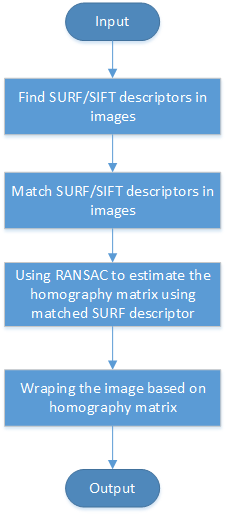
\includegraphics[height=0.9\linewidth]{extra-4}
	\centering
	\caption{\label{fig: extra-4}Image Mosaicing and Ortho-rectification process}
\end{figure}


\section{Image Mosaicing and Ortho-rectification}
The important steps in the algorithm are listed in Fig.~\ref{fig: extra-4} to give the reader an intuitive understanding.We need to stitch together our georeferenced images now to get an overall image of the farm land. This we can treat as the base map raster layer for our operations and we will perform a series of image processing algorithms on it to get pertinent data. The problem of image mosaicing is a combination of three problems:

\begin{enumerate}
	\item Correcting geometric deformations using image data and/or camera models.
	\item Image registration using image data and/or camera models.
	\item Eliminating seams from image mosaics.
\end{enumerate}

\subsection{Geometric corrections}
A geometric transformation could be a mapping that relocates image points. Transformations can be world or native in nature. Global transformations square measure sometimes outlined by a single equation that is applied to the complete image. Local transformations square measure applied to a half of image and those square measure tougher to specific briefly. 

The complications due to parallax that square measure determined within the case of change of location motion of a plate like camera are often avoided by employing a one dimensional camera to scan scenes. This action can be emulated victimization standard cameras by combining strips taken from a sequence of 2-D pictures as a series of neighboring segments. These cameras can directly acquire cylindrical (with a rotating motion) and writing (with change of location motion) maps. They can conjointly acquire pictures on Associate in nursing whimsical path. The strips that should be taken from 2-D pictures square measure known because the ones perpendicular to the image flow in. This family of strips can handle a wide form of motions together with motion and optical zoom. Additional formulation is developed in for these sophisticated cases of motion.

\section{Image Registration}
Image registration is the task of matching two or a lot of pictures. It has been a central issue for a range of problems in image process like seeing, monitoring satellite pictures, matching stereo images for reconstructing depth, matching biomedical pictures for designation, etc.

Registration is also the central task of image mosaicing procedures. The construction of mosaic images and the use of such images on several computer vision/graphics applications have been active areas of research in recent years. Carefully tag Associate in nursing pre-recorded camera parameters might be wont to eliminate the necessity for an automatic registration. User interaction also is a reliable supply for manually registering pictures (e.g. by choosing corresponding points and using necessary transformations on screen with visual feedback). Automated strategies for image registration used in image mosaicing literature will be categorized as follows:                                                                                                                                   

\begin{enumerate}
	\item Feature based methods
	\item Intensity based mosaicing
\end{enumerate}


\subsection{Feature based methods}

\begin{figure}[t]
	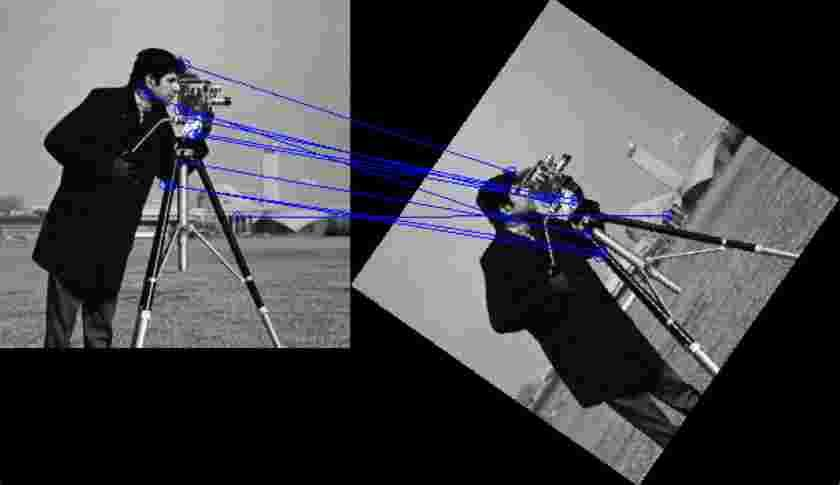
\includegraphics[width=0.9\linewidth]{extra-5}
	\centering
	\caption{\label{fig: extra-5}Feature based detection~\cite{FeatureD37:online}}
\end{figure}

In feature-based technique of Fig.~\ref{fig: extra-5}, all main feature points in an image pair is compare with all features in the other image by using one of the local descriptors. For image stitching based on feature-based techniques, feature extraction, registration, and blending are different steps required for doing image stitching. Feature-based methods are used by establishing correspondences between points, lines, edges, corners or any other shapes. The main characteristics of robust detectors includes invariance to image noise, scale invariance, translation invariance, and rotation transformations.

\subsection{Intensity based mosaicing}
Iteratively adjusting camera-motion parameters leads to local minimums unless a reliable initial estimate is provided. Initial estimates can be obtained using a coarse global search or an efficiently implemented frequency domain approach. Algorithm is as follows:

\begin{enumerate}
	\item For each pixel at ($x$, $y$) in the first image, we compute the corresponding pixel in the second image equal to ($x$', $y$').
	\item Compute the error density function between corresponding pixels.
	\item The problem is solved iterative to converge the error function towards the global minima.
\end{enumerate}

\section{Image Composting}
Images aligned once undergoing geometric corrections most seemingly need additional process to eliminate remaining distortions and discontinuities. Alignment of images might be imperfect as a result of registration errors ensuing from incompatible model assumptions, dynamic scenes, etc. Furthermore, in most cases images that want to be mosaiced don't seem to be exposed equally as a result of dynamical lighting conditions, automatic controls of cameras, printing/scanning devices, etc. These unwanted effects can be mitigated throughout the compositing method. 


The main downside in image compositing is that the problem of decisive however the pixels in Associate in nursing overlapping space ought to be delineated. Finding the best separation border between overlapping images has the potential to eliminate remaining geometric distortions. Such a border is likely to traverse around moving objects avoiding double exposure. The uneven exposure problem will be resolved by bar chart feat, by iteratively distributing the edge effect on the border to an outsized space, or by a smooth mixing perform.


\section{Ortho-Rectification of images}
The camera mounted on the drone is susceptible to different array of forces when the drone is airborne. This may result in changing of the orientation of the camera and hence the all the images may not be in the same plane. This can make the process of image mosaicing inaccurate and the final result we get will be a far off approximation of the real map of the field. To compensate for these errors, we need to implement some kind of pre-processing to account for this discrepancy in order to improve the efficiency of image mosaicing. Ortho-rectification is one of the ways to implement this compensation and is known to have good results for aerially acquired images. It is has an efficient implementation and so it requires less amount of processing time. This makes it compatible for real-world processing systems which is great advantage.
\begin{figure}[t]
	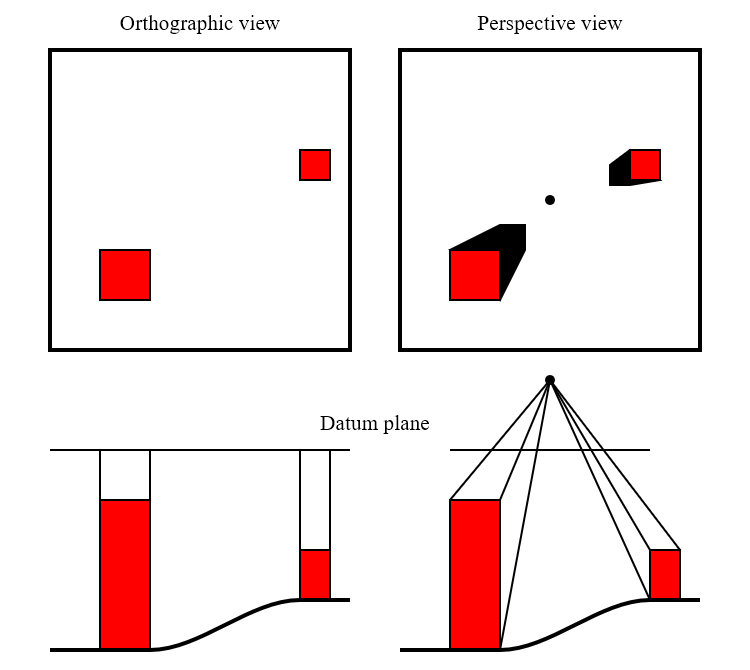
\includegraphics[height=0.9\linewidth]{extra-6}
	\centering
	\caption{\label{fig: extra-6}Ortho Rectification~\cite{OrthoPer57:online}}
\end{figure}
The process of ortho-rectification of Fig.~\ref{fig: extra-6} involves mapping of via aircraft non-inheritable pictures on a map of a similar size victimisation many geo-reference management points (GCPs)~\cite{1}. The topographical variations in the surface of  the world and also the tilt of the camera have an effect on  the gap with that options on the aerial image area unit show. The more topographically various the landscape, the more distortion inherent in the photograph. As a result, real world distances don't seem to be represented uniformly on the photograph. For example in a very steep area would relate to a way longer distance than an inch measured over a flat surface like a visible. Ortho-rectification is the name of the method accustomed removes these sources of distortion to equilibrate pic units with world distances. Once an aerial pic has been ortho-rectified, it is commonly cited as associate degree ortho-photo. A fascinating facet note is whereas ortho-rectification removes horizontal distortion; vertical relief displacement continues to be maintained. For example, the sides of a building would still contain distortion.

In some cases, a simple rectification method like removing the consequences of the lean of the camera is also all that's necessary. This is very rare and in most cases a lot of concerned method is needed. After removing the impact of the camera tilt, removing the effects of relief should be accomplished by knowing the elevation of the piece of land higher than (or below) the mapping plane must be identified~\cite{4}.

\subsection{Methods used in ortho-rectification}
There are two ways by that rectification of associate degree aerial photograph will occur. In the first case, Ground Control Points (GCP) are determined either typical ground surveys, from published maps, by Global Positioning System (GPS) surveys, or by aero triangulation. These points are taken at visible physical options on the landscape. On the corresponding image, the $x$, $y$ photo coordinates are then determined for every corresponding GCP. Depending on the sort of recursive correction to be used, a minimum of 3 to five GCP should be established. The relationship of the x, y photo coordinates to the real world GCP is then wont to confirm the algorithmic program for resampling the image.

The second method of ortho-rectification is to use DEMs. These elevations are collected from stereoscopic models by photogrammetric ways to kind a digital elevation model (DEM). As with using GCPs, the mathematical relationship between the real worlds coordinates and also the scanned aerial photograph is set and also the digital image is resampled to form the rectified image. For both cases, the resampling of the digital image involves warping the image thus that distance and space are uniform in relationship to world measurements. This means that with the resampled image, an in. on the image currently measures an equivalent distance on steep tract because it will during a field. Depending the on the desires of the aerial mental imagery within the GIS system, there are blessings and disadvantages to mistreatment either technique. GCP ortho-rectification is a faster method and may be accomplished mistreatment existing paper maps to ascertain the GCPs. Using DEMs for ortho-rectification is a lot of correct method by that to geocode digital mental imagery however need associate degree existing DEM or DTM for process. Once an image has been ortho-rectified it is often used with vector and formation information of an equivalent organization. This image can currently have broad outlines and street names overlay onto it. As mentioned before, spatial information will additionally currently be accurately measured in terms of distances and space, allowing for a lot of advanced spatial analysis~\cite{4}.

All the above mentioned method work separately for image mosaicing and ortho-rectification. We can use the SIFT (Scale Invariant Feature Transform) and SURF (Speeded-Up Robust Features) algorithms to simultaneously ortho-rectify the images and also stitch them. 

\section{SIFT and SURF}

\subsection{SIFT Detector}
\begin{figure}[h]
	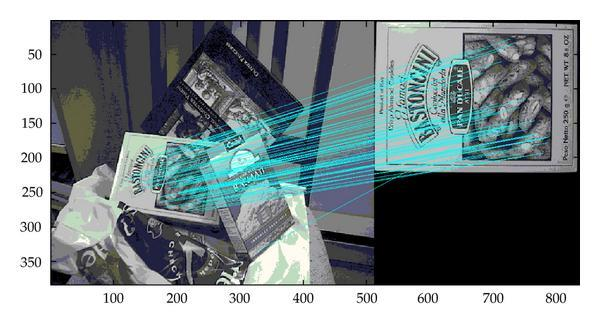
\includegraphics[width=0.9\linewidth]{extra-7}
	\centering
	\caption{\label{fig: extra-7}SIFT Based feature detection~\cite{FeatureM52:online}}
\end{figure}
Lowe proposed the Scale Invariant Feature remodel (SIFT). It has four computational phases that includes: scale-space extrema detection, key-point localization, orientation assignment, and defining key-point descriptors. The first stage is to spot location and scales of key point’s exploitation scale house extrema within the DoG (Difference-of-Gaussian) functions. In the key point localization Fig.~\ref{fig: extra-7} step, key point candidates are localized and refined by eliminating the key points wherever they rejected the low distinction points. In the orientation assignment step, the orientation of key point is obtained primarily based on native image gradient. In key-point descriptors stage, SIFT computes the local image descriptor for every key purpose supported image gradient magnitude and orientation at every image sample purpose in a very region focused at key purpose. These samples build a $3D$ histogram of gradient location and orientation, with $4$ X $4$ array location grid and eight orientation bins in each sample. SIFT provides a $128$-element dimension of key point descriptor. 

\subsection{SURF Detector}

The Speed-up Robust Feature detector (SURF) rule is based mostly on multiscale area theory and Speeds-up its computations by quick approximation of boot matrix and descriptor exploitation ``integral images''. SURF uses three feature detection steps namely; detection, description, and matching. SURF speeded-up the SIFT’s detection process by keeping in read of the standard of the detected points Fig.~\ref{fig: extra-8}. It gives a lot of focus on speeding-up the matching step~\cite{5}. The Hessian matrix is used alongside descriptors low spatial property to considerably increase the matching speed. SURF is widely used in the pc vision community. SURF has proven its potency and hardiness in the invariant feature-localization. 
\begin{figure}[h]
	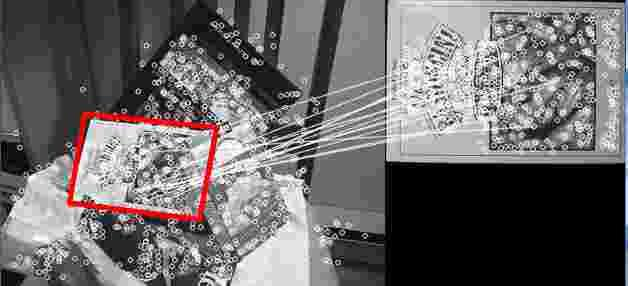
\includegraphics[width=0.9\linewidth]{extra-8}
	\centering
	\caption{\label{fig: extra-8}SURF Based feature based detection~\cite{FeatureD76:online}}
\end{figure}

\section{OpenDronemap based Image Processing}

OpenDroneMap is a tool to postprocess drone, balloon, kite, and street view data to geographic data including orthophotos, point clouds, \& textured mesh.

Docker is the world’s leading software container platform. Developers use Docker to eliminate ``works on my machine'' problems when collaborating on code with co-workers. Using containers, everything required to make a piece of software run is packaged into isolated containers. Unlike VMs, containers do not bundle a full operating system - only libraries and settings required to make the software work are needed.

We used opendronemap to achieve the step of image stitching robustly. We used docker as a container for easier installation and cross-platform support across all different OS and platforms. 

The main command to start the procedure is:

\begin{lstlisting}
docker build -t opendronemap:latest
\end{lstlisting}

This command builds the docker image using dockerfile. This command also creates a container that is used to generate the stitched image using georef coordinates.

\begin{lstlisting}
`docker run -it --rm -v img_loc:/code/images -v odm_orthophoto:/code/odm_orthophoto -v 
/odm_texturing:/code/odm_texturing my_odm_image_2`
\end{lstlisting}


